\documentclass[pdf]{beamer}
\usetheme{Copenhagen}
\usepackage{multicol, latexsym, amsmath, amssymb}
\usepackage{smartdiagram}
\usepackage{subcaption}
\usepackage{graphics}
\usepackage{xcolor}
\usepackage[absolute,overlay]{textpos}

\graphicspath{{./images/}}

\setbeamertemplate{navigation symbols}{}

\setbeamercolor{framesource}{fg=gray}
\setbeamerfont{framesource}{size=\tiny}
\newcommand{\source}[1]{\begin{textblock*}{4cm}(8.7cm,8.6cm)
    \begin{beamercolorbox}[ht=0.5cm,right]{framesource}
        \usebeamerfont{framesource}\usebeamercolor[fg]{framesource} Source: {#1}
    \end{beamercolorbox}
\end{textblock*}}

\title[Descent-to-Delete]{Descent-to-Delete:\\ Gradient-Based Methods for Machine Unlearning}
\subtitle[]{Seth Neel, Aaron Roth, Saeed Sharifi-Malvajerdi}

\author[Neel et al.]{Presented by Ananth Mahadevan}
\date{\today}

\begin{document}
\begin{frame}
    \titlepage
\end{frame}

\begin{frame}
    \frametitle{Contents}
    \tableofcontents
\end{frame}

\section{Unlearning}
\subsection{Motivation}
\begin{frame}
    \frametitle{Data Removal}
    \begin{itemize}
        \item Right to be Forgotten and GDPR
        \item Deleting personal data from datasets
        \item How to remove influence of data on deployed ML models? Retrain them on remaining sample?
        \item Retraining effort is disproportionate to number of deletion requests
    \end{itemize}
    \begin{block}<1->{Problem Statement}
        Design an efficient \textbf{unlearning algorithm} that produces model outputs that are \textbf{statistically indistinguishable} from the model outputs that would have arisen from \textbf{retraining}
    \end{block}
    

\end{frame}
\subsection{Differential Privacy Unlearning}
\begin{frame}
    \frametitle{}
    \begin{figure}
        \centering
        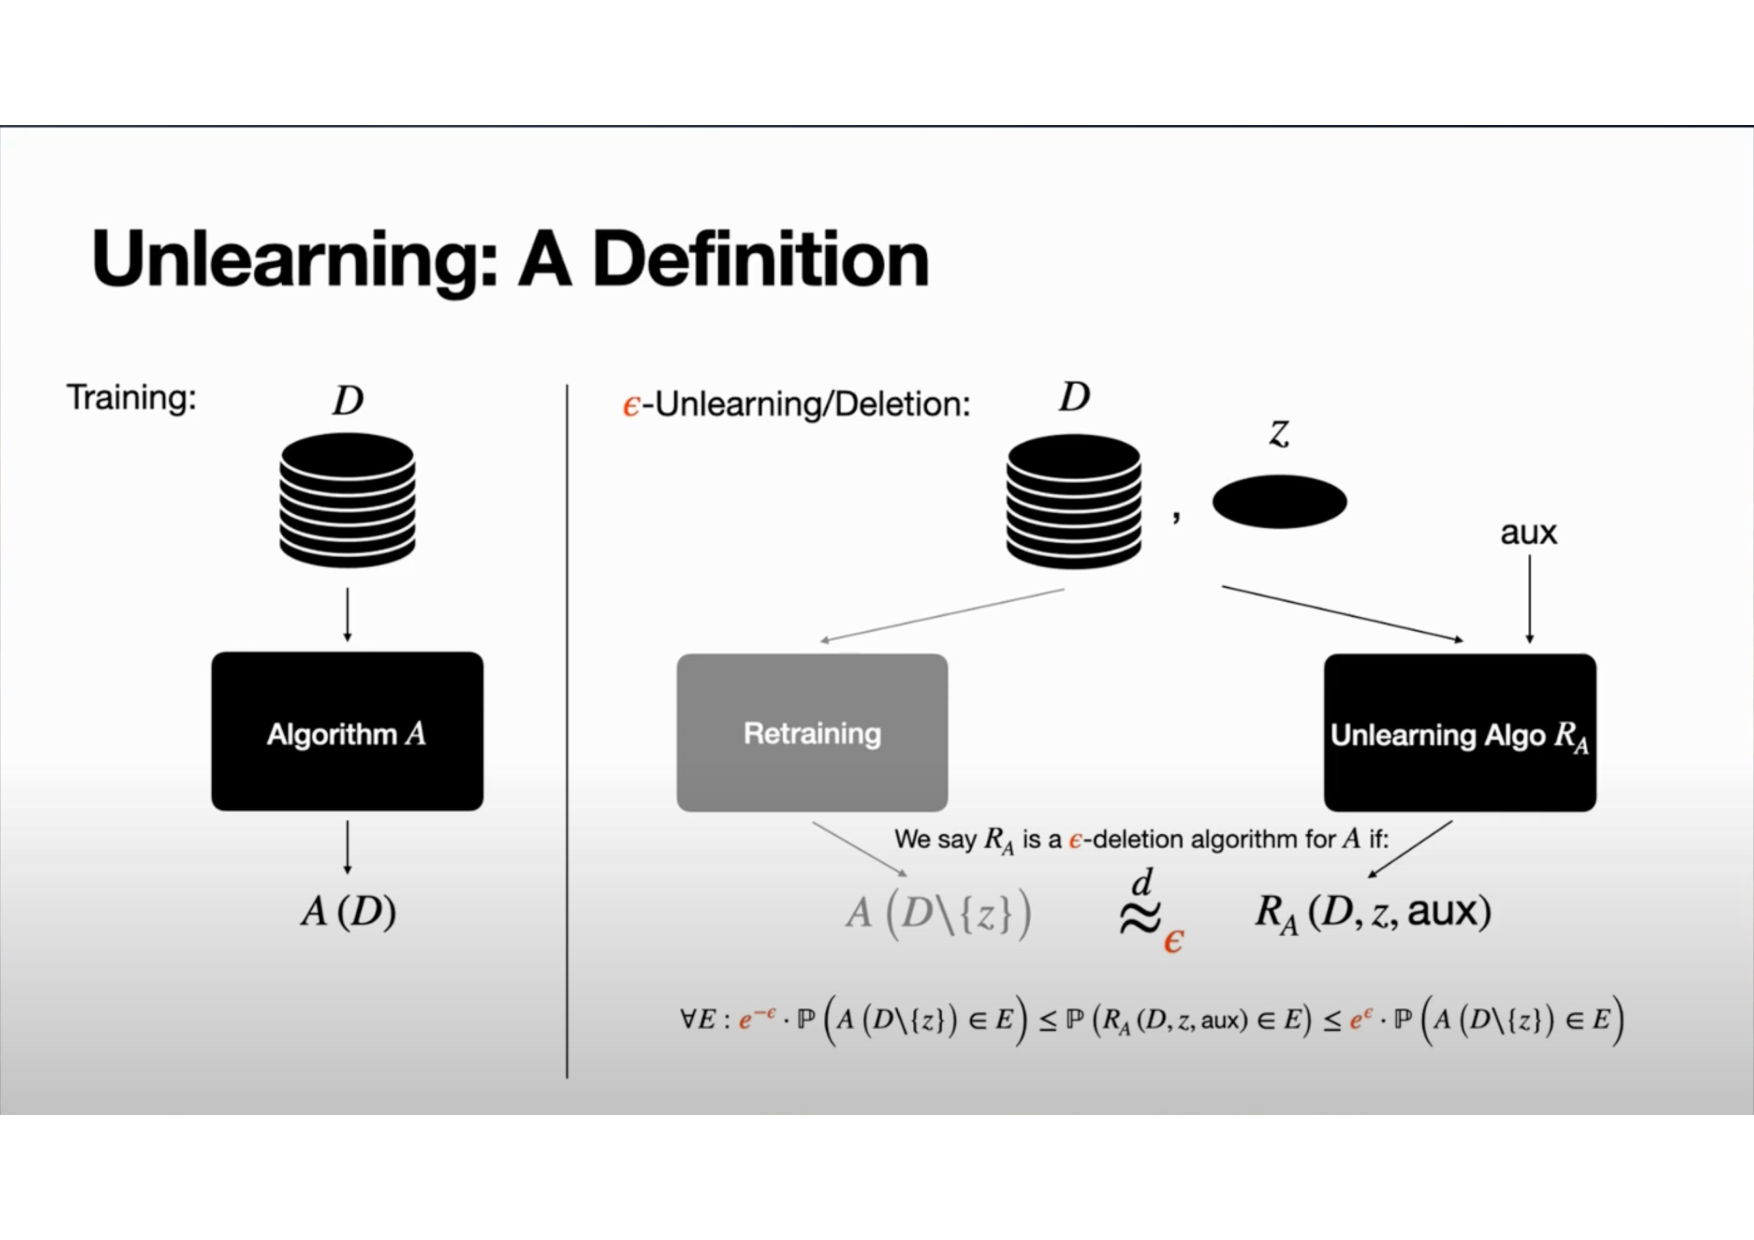
\includegraphics[trim={1cm 2cm 2cm 2cm},clip,width=1.05\textwidth]{unlearning.pdf}
        \source{ALT Youtube Channel}
    \end{figure}

\end{frame}

\begin{frame}
    \frametitle{Preliminaries}
    \begin{itemize}
        \item<1-> Original dataset $\mathcal{D}_0$ and after $i$th removal $\mathcal{D}_i$ 
        \item<2-> \textbf{Learning} algorithm $\mathcal{A}$ and $\mathcal{A}(\mathcal{D}_{0})=\theta_{0}$
        \item<3-> \textbf{Unlearning} algorithm for $\mathcal{A}$, $\mathcal{R}_{\mathcal{A}}$ 
        \item<4-> For $i\geq 1$ and removal $z_i$, $\mathcal{R}_{\mathcal{A}}(\mathcal{D}_{i-1},z_{i},\textcolor<5->{red}{\theta_{i}})=\hat{\theta}_{i}$
        \item<6-> \textbf{Publishing function} $f_{\text{publish}}$ adds i.i.d gaussian noise with $0$ mean and $\sigma$ variance
        \item<7-> $f_{\text{publish}}(\theta_{0})=\tilde{\theta}_{0}$ and $f_{\text{publish}}(\hat{\theta}_{i})=\tilde{\theta}_{i}$ when $i\geq1$
        \item<8-> Simply, $\{\hat{\theta}_{i}\}_{i\geq 1}$ are \textbf{secret} model outputs and $\{\tilde{\theta}_{i}\}_{i\geq 0}$ are \textbf{public} models
    \end{itemize}
    

\end{frame}
\subsection{Categorization of Unlearning}
\begin{frame}
    \frametitle{Perfect vs \textit{Imperfect}? Unlearning}
    Perfect Unlearning Algorithm
    \begin{itemize}
        \item Requires indistinguishable wrt \textbf{full internal state} 
        \item \textbf{Stronger} requirement, similar to \emph{pan privacy} in differential-privacy
        \item Unlearning algorithm $\mathcal{R}_{\mathcal{A}}$ uses \textbf{published model as input} at each step, i.e.\ $\theta_{i} = \tilde{\theta}_{i-1}$
        \item All prior work focus on perfect unlearning algorithms
    \end{itemize}
\end{frame}

\begin{frame}
    \frametitle{Perfect vs \textit{Imperfect}? Unlearning}
    Imperfect? Unlearning
    \begin{itemize}
        \item Requires only statistical indistinguishability wrt \textbf{observed outputs} of algorithm
        \item Allowed to maintain a ``\textbf{secret state}'' for unlearning
        \item Secret state need not satisfy indistinguishability requirement
        \item Unlearning algorithm $\mathcal{R}_{\mathcal{A}}$ maintains previous step's output $\hat{\theta}_{i-1}$ as secret state
        \item This is used as input at the current step $i$, i.e.\ $\theta_{i}=\hat{\theta_{i-1}}$
    \end{itemize}
\end{frame}

\begin{frame}
    \frametitle{Strong and Weak Unlearning}
    \begin{block}<1->{Strong Unlearning Algorithm}
        For a fixed accuracy target,
        the run-time of the update operation be constant (or at most logarithmic) 
        in the length of the update sequence.
    \end{block}
    \begin{block}<2->{Weak Unlearning Algorithm}
        It may have run-time per update (or equivalently, error)
        that grows polynomially with the length of the update sequence
    \end{block}
    

\end{frame}

\section{ERM Framework}
\begin{frame}
    \frametitle{Empirical Risk Minimization Framework}
    \begin{itemize}
        \item Convex loss function $\ell: \mathbb{R}^{d} \times Z \rightarrow \mathbb{R}$.
        \item Dataset $D=\left\{z_{1}, z_{2}, \ldots, z_{n}\right\} \in Z^{n}$
        \item Want to solve: $\min _{\theta \in \mathbb{R}^{d}} \frac{1}{n} \sum_{i=1}^{n} \ell\left(\theta, z_{i}\right):=\mathcal{L}(\theta, D)$
        \item Algorithm: Gradient Descent: $\theta_{0}, \forall t \leq T: \theta_{t}=\theta_{t-1}-\eta \nabla L\left(\theta_{t-1}, D\right)$
        \item Computation cost: number of iterations T
        \item Accuracy: $\mathcal{L}\left(\theta_{T}, D\right)-\min _{\theta} \mathcal{L}(\theta, D)$
    \end{itemize}
    

\end{frame}

\section{Perturbed Gradient Descent}
\subsection{Strong Convexity}
\begin{frame}
    \frametitle{Covergence Results for Gradient Descent}
    \begin{block}{Strongly Convex and Smooth}
        
         Let $\ell$ be $m$-strongly convex and $M$ smooth, and let $\theta^{*}=\operatorname{argmin}_{\theta \in \Theta} \mathcal{L}(\theta) .$ We have that after $T$ steps of $G D$ with step size $\eta_{t}=\frac{2}{m+M}$,
            $$\left\|\theta_{T}-\theta^{*}\right\|_{2} \leq\left(\frac{M-m}{M+m}\right)^{T}\left\|\theta_{0}-\theta^{*}\right\|_{2}
            $$
    \end{block}

\end{frame}

\begin{frame}
    \frametitle{Differential Privacy Sensitivity}
    \begin{block}{Sensitivity}
        Suppose $\ell$ is $L$ -Lipschitz and $m$ -strongly convex. For any dataset $\mathcal{D}$, let $\theta_{\mathcal{D}}^{*} \triangleq \operatorname{argmin}_{\theta \in \Theta} \mathcal{L}(\theta) .$ We have that for any integer $n$, any data set $\mathcal{D}$ of size $n$, and any removal $z\in \mathcal{D}$,
        $$\left\|\theta_{\mathcal{D}}^{*}-\theta_{\mathcal{D} \setminus \{z\}}^{*}\right\|_{2} \leq \frac{2 L}{m n} .$$
   \end{block}

\end{frame}
\begin{frame}
    \frametitle{Perturbed Gradient Descent}
    \begin{figure}
        \centering
        \def\svgwidth{\columnwidth}
        \scalebox{0.5}{\input{images/image2.pdf_tex}}
        \source{Chris Waites' Blog}

    \end{figure}
\end{frame}
\begin{frame}
    \frametitle{Perturbed Gradient Descent}
    \begin{figure}
        \centering
        \def\svgwidth{\columnwidth}
        \scalebox{0.5}{\input{images/image1.pdf_tex}}
        \source{Chris Waites' Blog}

    \end{figure}
\end{frame}
\begin{frame}
    \frametitle{Perturbed Gradient Descent}
    \begin{figure}
        \centering
        \def\svgwidth{\columnwidth}
        \scalebox{0.5}{\input{images/image3.pdf_tex}}
        \source{Chris Waites' Blog}

    \end{figure}
\end{frame}
\begin{frame}
    \frametitle{Perturbed Gradient Descent}
    \begin{figure}
        \centering
        \def\svgwidth{\columnwidth}
        \scalebox{0.5}{\input{images/image4.pdf_tex}}
        \source{Chris Waites' Blog}

    \end{figure}
\end{frame}
\begin{frame}
    \frametitle{Perturbed Gradient Descent}
    \begin{figure}
        \centering
        \def\svgwidth{\columnwidth}
        \scalebox{0.5}{\input{images/image5.pdf_tex}}
        \source{Chris Waites' Blog}

    \end{figure}
\end{frame}
\begin{frame}
    \frametitle{Perturbed Gradient Descent}
    \begin{figure}
        \centering
        \def\svgwidth{\columnwidth}
        \scalebox{0.5}{\input{images/image6.pdf_tex}}
        \source{Chris Waites' Blog}

    \end{figure}
\end{frame}
\subsection{Convexity}
\begin{frame}
    \frametitle{Regularized Perturbed Gradient Descent}
    \begin{itemize}
        \item When $\ell$ is not strongly convex, can regularize it to enforce strong convexity
        \item Regularized loss: $\mathcal{L}_m(\theta,D) = \mathcal{L}(\theta,D)+\frac{m}{2}\|\theta\|_{2}^{2}$
        \item Issues with aggressive regularization 
        \begin{itemize}
            \item $m\uparrow~\longrightarrow\text{sensitivity}\downarrow~\longrightarrow\text{perturbation}\downarrow~\longrightarrow\text{accuracy}\uparrow$
            \item $m\uparrow~\longrightarrow L(\theta_{T},D)\uparrow~\longrightarrow\text{accuracy}\downarrow$
            \item $m\uparrow~\longrightarrow\text{Degrades Lipschitz/smoothness of loss functions}$
        \end{itemize}
        \item Therefore regularization needs to be chosen carefully
    \end{itemize}
\end{frame}
\subsection{Distributed Setting}
\begin{frame}
    \frametitle{Perturbed Distributed Descent}
    High Level Idea
    \begin{itemize}
        \item Randomly partition dataset into $K$ parts
        \item Train models separately on each part to minimize empirical loss
        \item Take the average of $K$ models 
        \item Publish average model after adding noise  
    \end{itemize}
    Benefits 
    \begin{itemize}
        \item \cite{JMLR:v14:zhang13b} provides \textit{out of sample guarantee} for accuracy of distributed setting
        \item Removed element present in some partition, update only those partition
        \item Improved results given same computation budget as non-distributed
    \end{itemize}

\end{frame}

\section{Results}
\begin{frame}
    \frametitle{Results}
    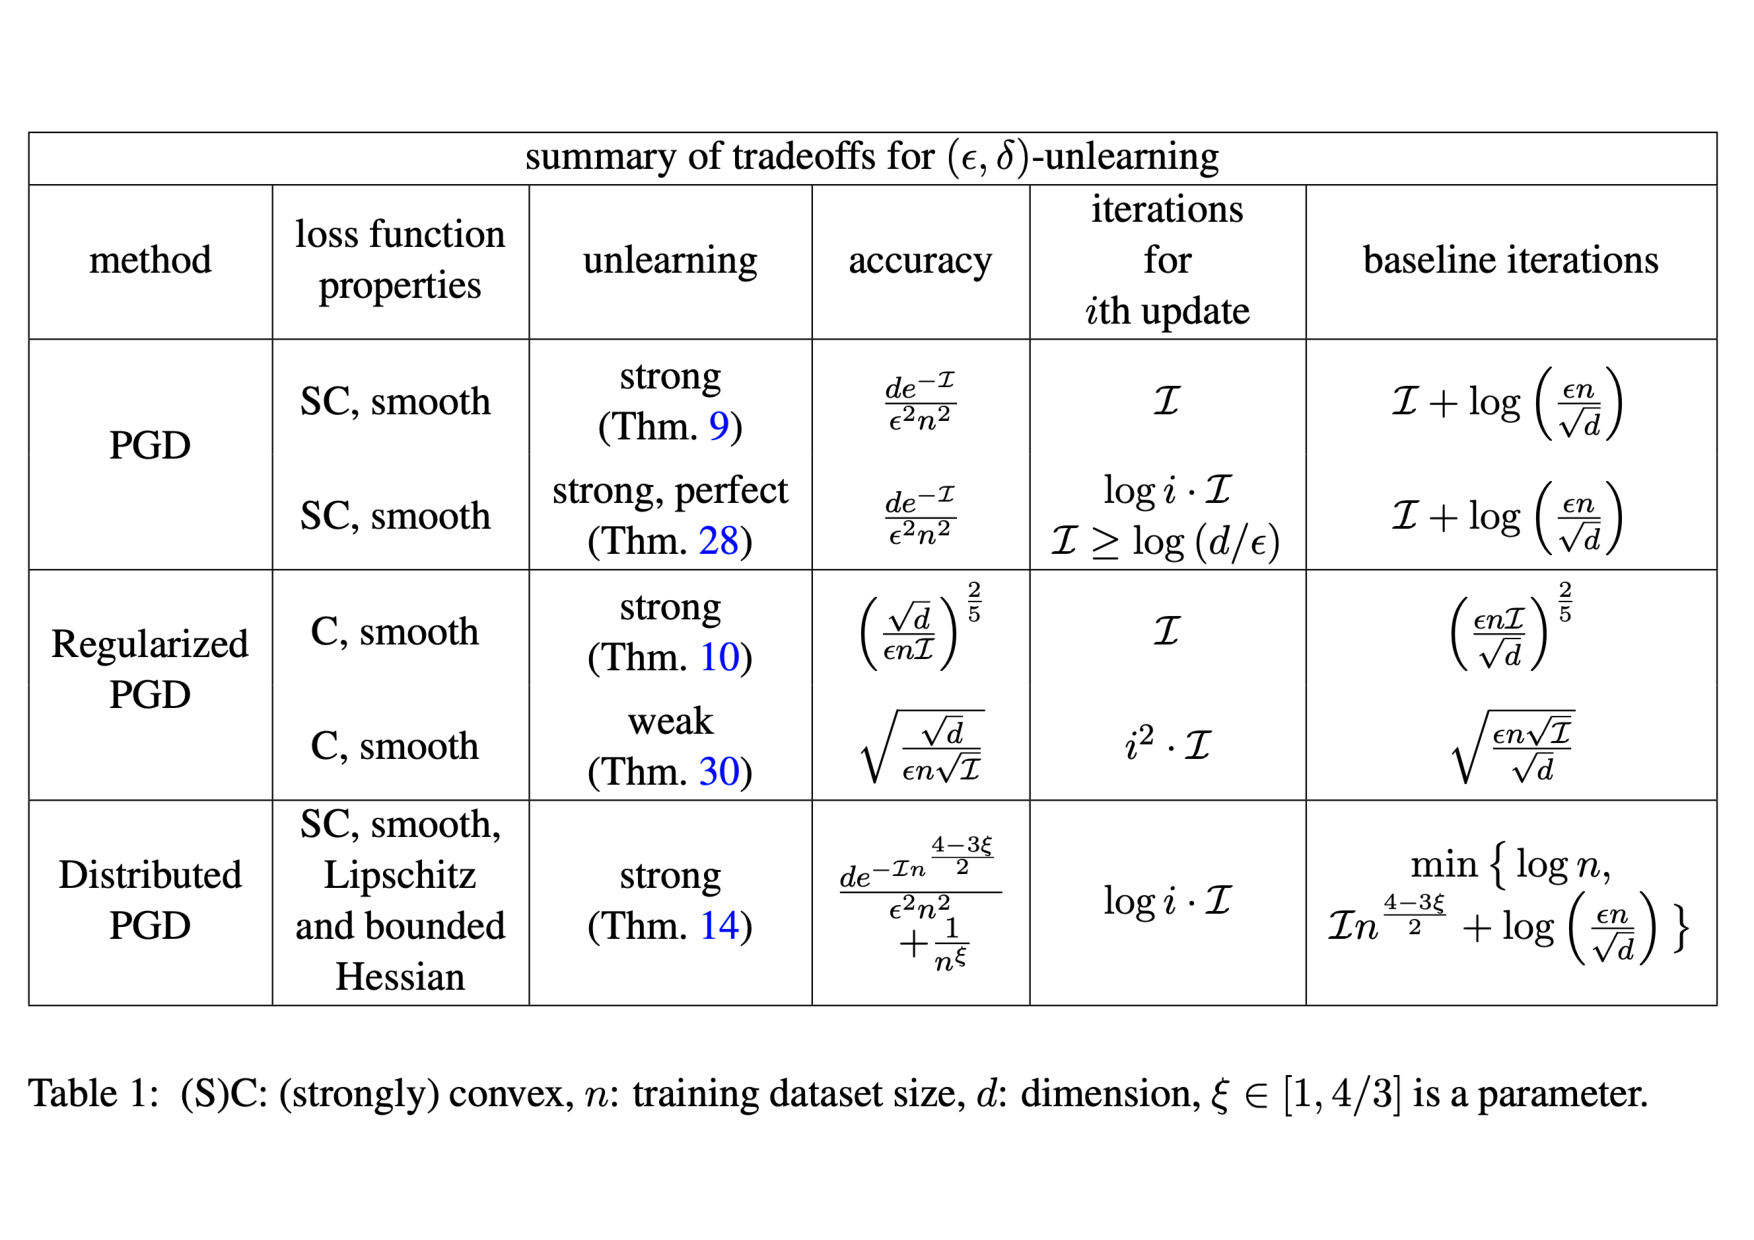
\includegraphics[width=\textwidth]{results.pdf}
\end{frame}
\section{Future Ideas}
\begin{frame}
    \frametitle{Future Directions}
    \begin{itemize}
        \item Extensive experiential analysis to check practical feasibility
        \item Extend approach to SGD with similar analysis in \cite{wuDeltaGradRapidRetraining2020}
        \item Check for local convexity in Neural Network loss landscapes and extend approach
    \end{itemize}
\end{frame}


\begin{frame}[allowframebreaks]
    \frametitle{References}
    \bibliography{references}
    \bibliographystyle{alpha}
\end{frame}
  

\end{document}